\section{Results}
\label{sec:results}

In the following sections, we explore the response of the log-loss and Brier score metrics to the classifiers of Section~\ref{sec:data} and as a function of the weights on affected classes.

\subsection{Mock classifier systematics}
\label{sec:mockresults}

We simulate probabilistic classifications as potential submissions to \plasticc\ by the methodology of Section~\ref{sec:mockdata} based on CPMs composed of pairs of the characteristic classifiers shown in Figure~\ref{fig:all_combined} under various weightings described below.

\begin{figure*}
	\begin{center}
		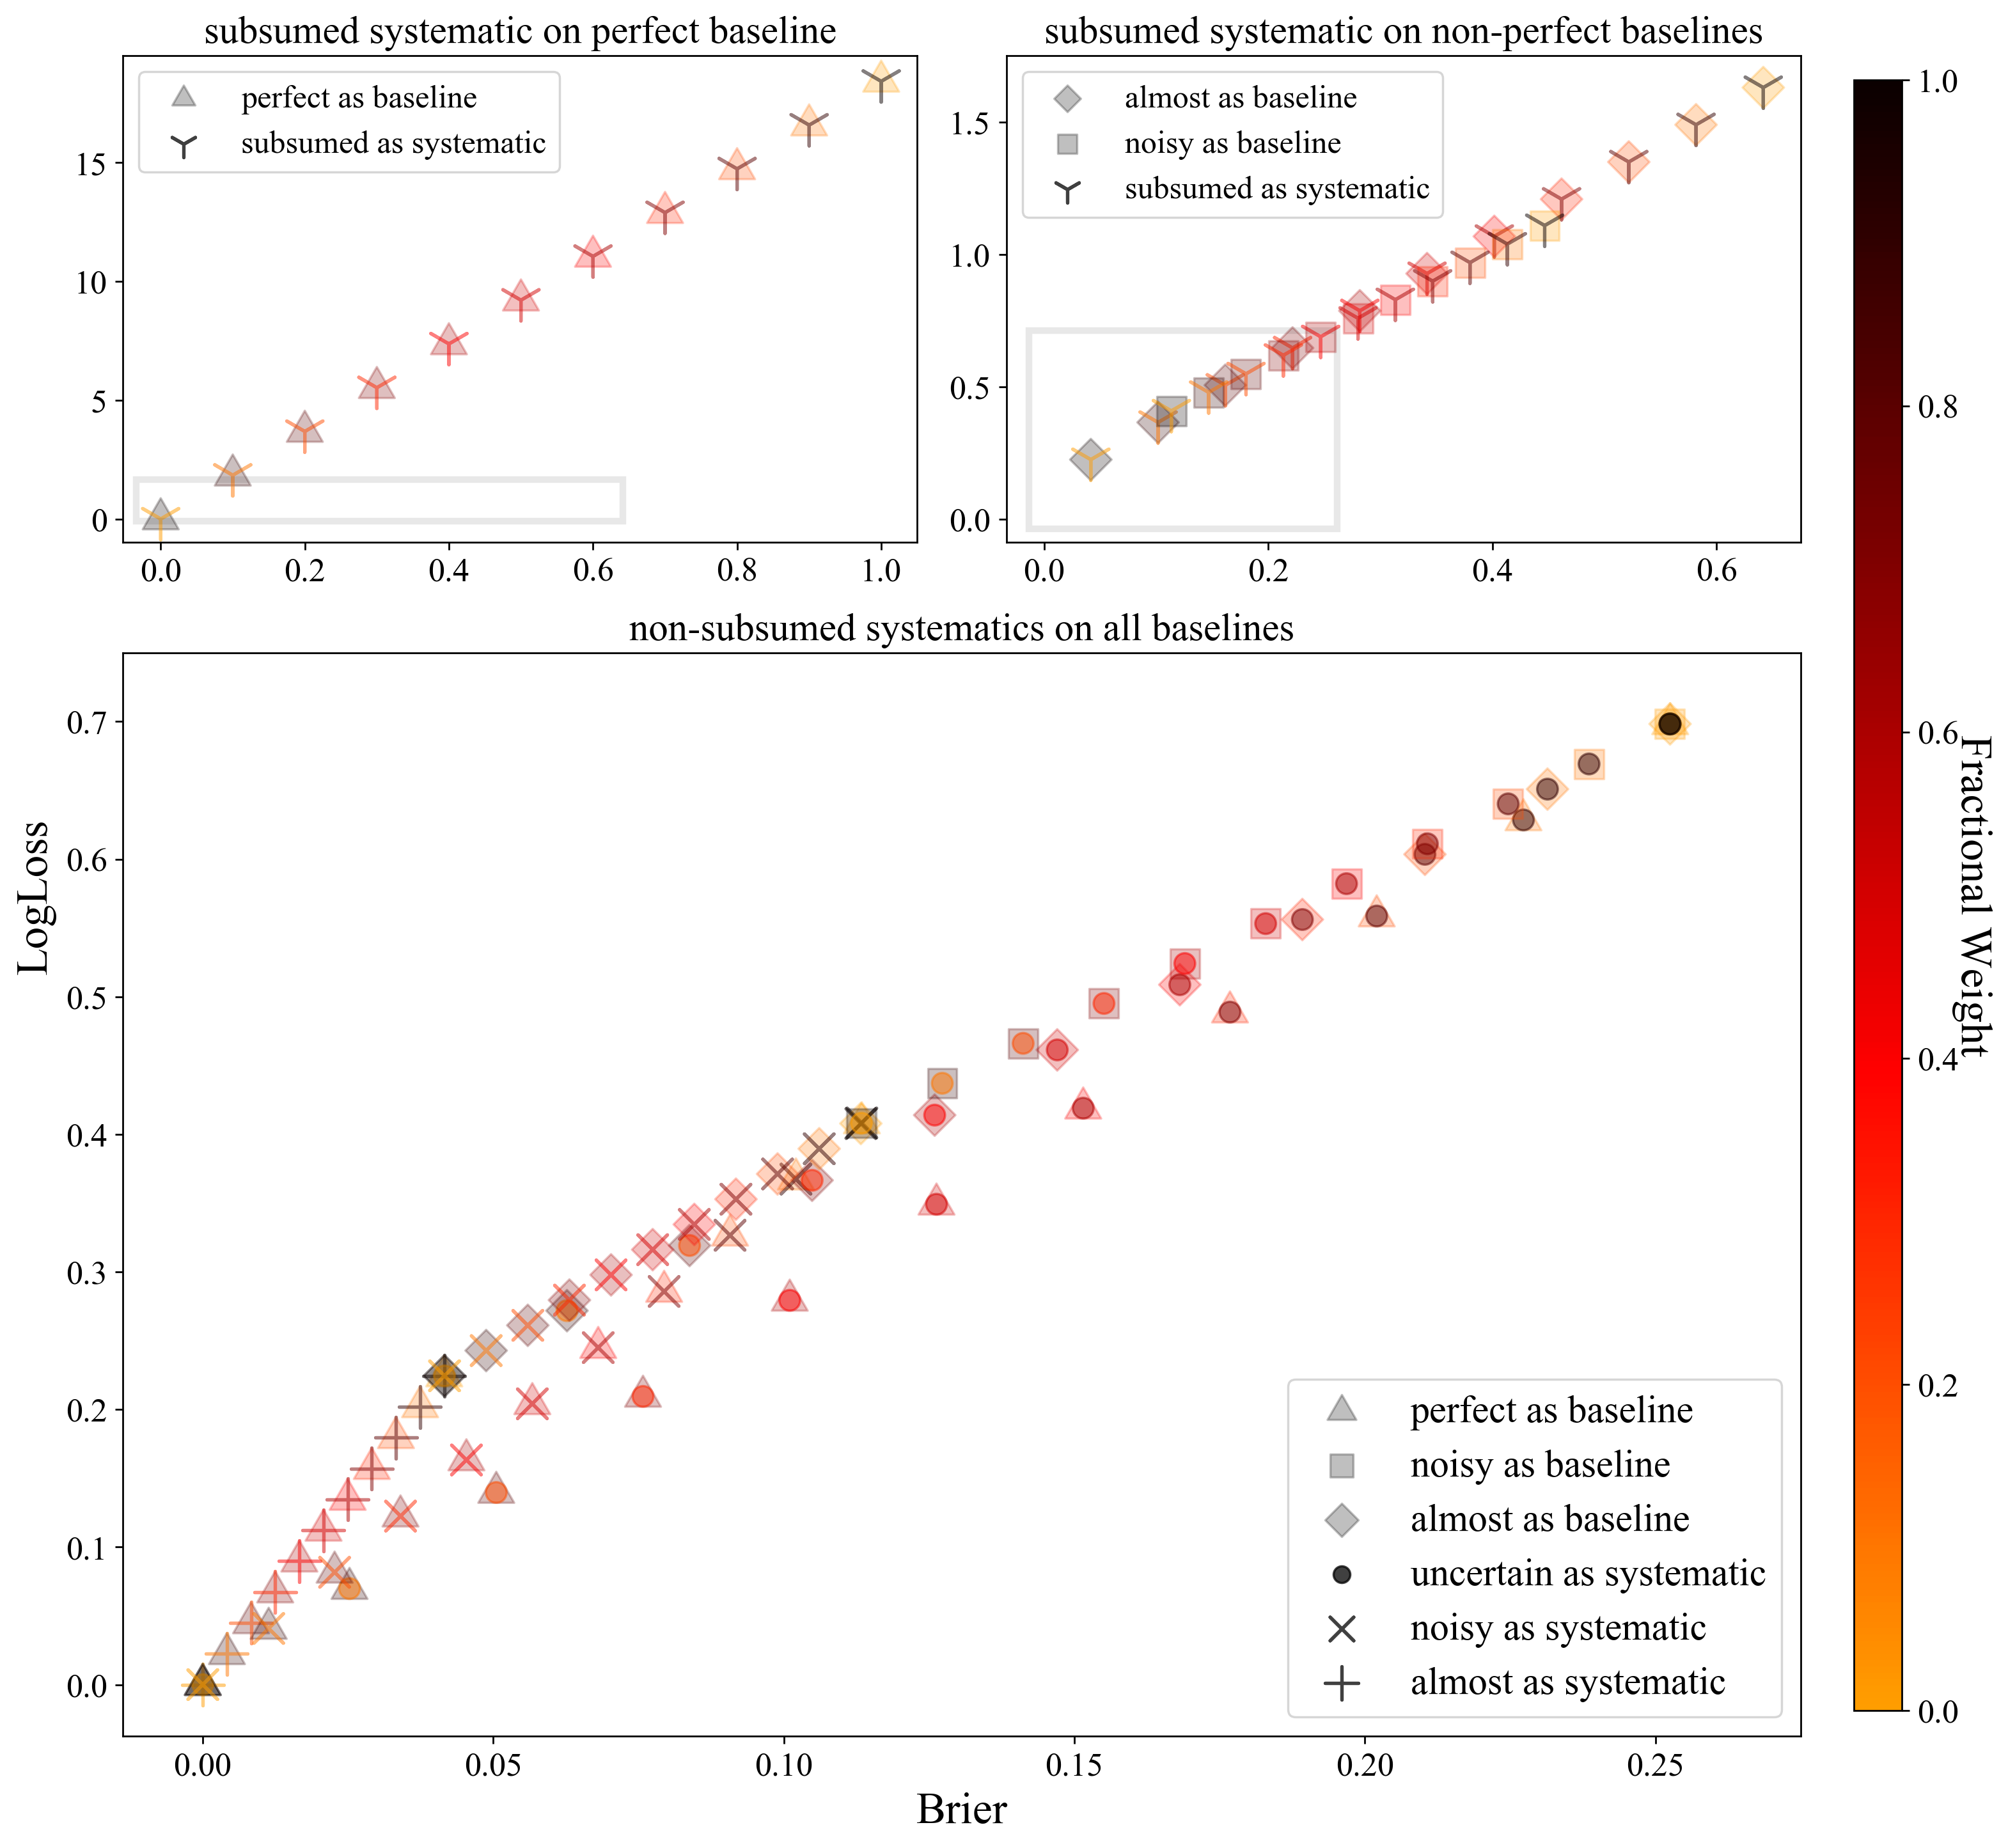
\includegraphics[width=0.99\textwidth]{./fig/multipanel_res.png}
		\caption{
		Weighted log-loss and Brier scores for baseline classifiers with combinations of systematics.
		Each point represents a classifier with a shared baseline behavior (regular polygon marker; triangle for perfect, diamond for almost perfect, square for noisy) for all but one class, which is affected by a particular systematic (asterisk markers; plus for almost perfect, cross for noisy, dot for uncertain, and Y-shape for subsumed).
		The color of the marker for the systematic effect indicates the weight on the one class affected by that systematic, while the color of the baseline behavior marker indicates the integrated weight evenly distributed over other classes with baseline behavior, where lower weights are greener and higher weights are bluer.
		From left to right, we zoom in on a particular range of scores, to highlight the scale of the effect of weighted systematics on the metrics for well-behaved methods with low Brier/log-loss values.
		The ranges of Brier score and log-loss values between the panels are in ratios of approximately 10:7:3 and 100:10:5, respectively, indicating the log-loss's higher sensitivity to the presence of systematics.
		The metrics are most sensitive to the subsuming systematic on a perfect baseline (triangle with Y-shaped marker), whereas other combinations of baseline and systematic can be grouped with a smaller dynamic range in both metrics.
		}
	\end{center}
	\label{fig:all_combined}
\end{figure*}

The systematics introduced to each baseline are those that we intuitively expect to worsen classification performance of an arbitrary classifier:
\begin{itemize}
\item the uncertain, almost perfect, noisy, and subsuming classifiers are anticipated to worsen an otherwise perfect classifier;
\item the uncertain, noisy, and subsuming classifiers are anticipated to worsen an otherwise almost perfect classifier;
\item the uncertain and subsuming classifiers are anticipated to worsen an otherwise noisy classifier.
\end{itemize}
In every case, we apply the systematic to one true class, which corresponds to transforming one row of the baseline CPM.

The introduction of weights illustrates the effect each particular systematic has on a given baseline, and more importantly, how up- (or down-) weighting the affected class changes the overall metric value for the mock classifier.
Weighting schemes are defined by a weight $0 \leq w \leq 1$ on the affected class, with the remaining baseline classes sharing equal weight $(1 - w) / (M - 1)$; we test eleven weighting schemes with $w = 0., 0.1, \dots, 1.$.
A higher weight on the systematic corresponds to a lower weight on the more desirable baseline, causing both the log-loss and Brier score to increase.
This variation in weights establishes linear relationships between the log-loss and Brier score metrics for each pair of baseline and systematic, but the slope is related to the relative sensitivity of the metrics.

Figure~\ref{fig:all_combined} confirms that for all weight on the perfect classifier, the values of both metrics vanish to zero.
It is worth noting that the log-loss has more dynamic range than the Brier score overall, and that the log-loss is acutely sensitive to the subsuming systematic on a baseline of a perfect classifier.
However, the relative scales of metric values for different baseline-plus-systematic pairs are quite large, requiring three panels, zooming in from left to right.

The left panel of Figure~\ref{fig:all_combined} shows the largest variations in metric scores, for the combination of the perfect baseline and a subsuming systematic where one class is given a probability of 1 for being in another particular class and a probability of 0 for being in its true class.
This means both metrics are acutely sensitive to the subsuming systematic on a perfect baseline, which can only be overcome by aggressive downweighting.
In fact, the log-loss value for a classifier that subsumes a class into one that is classified perfectly should be infinite if the classes unaffected by the systematic have no weight; it is only finite for us because of the limits of numerical precision.

The middle panel of Figure~\ref{fig:all_combined} illustrates a narrower range of log-loss and Brier score for the subsuming systematic on the almost perfect and noisy classifier baselines.
The subsuming systematic on any baseline besides the perfect classifier defines a new regime of high but not infinite values of the metrics.

The right panel of Figure~\ref{fig:all_combined} shows the values for all other systematics on all baselines.
Though the slope is lower than in the other panels, the dynamic range of the log-loss remains higher; in other words, the log-loss is in general more sensitive to systematics than the Brier score.

In summary, both the log-loss and Brier score are most sensitive to the subsuming systematic than any other systematic.
Tuning the weights can provide an avenue toward imposing a global metric penalty on classifiers exhibiting a systematic on one class.

\begin{table}[]
\begin{tabular}{lll}
Classifier characteristic & Brier score & Log-loss\\
\hline
Perfect & 0.0 & 0.0\\
Almost perfect & 0.042 & 0.225\\
Noisy & 0.113 & 0.408\\
Uncertain & 0.253 & 0.699\\
Subsumed from Noisy & 0.447 & 1.109\\
Subsumed from Almost & 0.641 & 1.629\\
Subsumed from Perfect & 1.0 & 18.421\footnote{The entry for the log-loss of a classifier that subsumes a class into one that is otherwise perfectly classified should be infinite but is bounded by the numerical precision of our calculations.}
\end{tabular}
\caption{\sout{The value of each metric when the weight is entirely on the class with the indicated characteristic.
Weighting changes the metric performance: the value of each metric when the weight is entirely on the class with the indicated characteristic (\changes{corresponding} to a $w=1$ case in Figure~\ref{fig:all_combined}).
The log-loss is more sensitive than \changes{the} Brier score, with larger values of the score (indicating poor classification performance), particularly for the subsuming systematic.}
\changes{Metric values computed using Equation~\ref{eq:weightavg} with unit weights for the mock data produced by mock classification schemes described in Sec.~\ref{sec:mockdata}.
While the log-loss metric has a larger dynamic range than the Brier score for poor classification, the toy classifiers would be ranked the same way by either metric.}
}
\label{tab:extents}
\end{table}

When all weight is on the class exhibiting the systematic, there is a characteristic limit for each metric's values, shown in Table~\ref{tab:extents}.
Because a subsumed class takes the conditional probability vector of the subsuming class, the metric values depend on what systematics may be affecting the subsuming class as well.
While the two metrics obviously take different values, in accordance with their slopes given in Table~\ref{tab:slopes}, they do agree on the ranking of these classifiers.
Though this agreement is not in general guaranteed, it is a desirable behavior, indicating that these metrics would lead to the same conclusion about the severity of each systematic.

\begin{table}[]
\begin{tabular}{l|llll}
	& Systematics & & &\\
Baselines & Subsumed & Uncertain & Noisy & Almost\\
\hline
Perfect & 18.421 & 2.763 & 3.601 & 5.387\\
Almost perfect & 2.343 & 2.246 & 2.556 & \\
Noisy & 2.102 & 2.085 & &
\end{tabular}
\caption{
The slopes for each baseline-plus-systematic pair in the space of log-loss versus Brier score.
A higher slope corresponds to increased sensitivity of the log-loss over the Brier score.
The contrast between log-loss and Brier score is highest on a baseline of the perfect classifier, meaning the log-loss may be more appropriate for discriminating between classifiers that are already extremely good.
}
\label{tab:slopes}
\end{table}

The relative sensitivity ratios of the log-loss to the Brier score are the slopes in the trends of Figure~\ref{fig:all_combined} and are given in Table~\ref{tab:slopes}.
The log-loss always has higher sensitivity than the Brier score (i.e. it responds more strongly to up-weighting classes affected by a systematic), particularly to the difference between the perfect classifier and any lesser classifier.
A possible implication of this behavior is that the log-loss may have an enhanced ability to distinguish between multiple high-performing classifiers that might not have meaningfully different metric values under the Brier score.

On the other hand, the log-loss can be seen as more susceptible to the tunnel vision classifier because its value improves sharply with any move toward perfection.
If the subsumed class has little weight, the metric values are quite low, moreso for the log-loss than the Brier score.
This means that under a population-proportional weighting scheme, it would not be penalized for subsuming an uncommon class if it performed well for a more common class, a situation that would not serve the needs of the astronomical community.

% \aim{Still reworking past here.}
% Consider a weighting of $\sim0.8$ for a class affected by tunnel vision, leaving $\sim0.2$ to be shared evenly among all other classes uniformly affected by the other systematics.
% Qualitatively, we would say that a classifier that is almost perfect for other classes is superior to one that is noisy, and a classifier that is noisy for other classes is still superior to one that is uniform; furthermore, the subsuming classifier is even more harshly penalized in this situation than the uncertain classifier, meaning both metrics are  consistent with our basic tests of intuition in this case.
% However, this observation also indicates that the tunnel vision systematic is difficult to penalize, and that if the affected class is given a large weight, it can easily dominate the metric.
% If all classes are of scientific importance, heavily unequal weighting can incentivize tunnel vision classification.

% We introduced weighting of per-class metrics to discourage `tunnel vision' and `cruise control' classifiers that can ignore classes other than the most common and nonetheless perform well by a metric.
% Figure~\ref{fig:popweight} shows the impact of weighting the per-class metrics by the number of objects in the class as each is affected by one of the systematics and the other classes are held at the more realistic almost perfect performance.
% The points show different classification schemes, and all points are coloured by the change in the weighting, dependent on the size of the population class being classified.
% Conversely, the cruise control classifier and, to a lesser degree the noisy classifier, always has high log-loss and Brier score values regardless of the weight on the affected class.

% \begin{figure}
% 	\begin{center}
% 		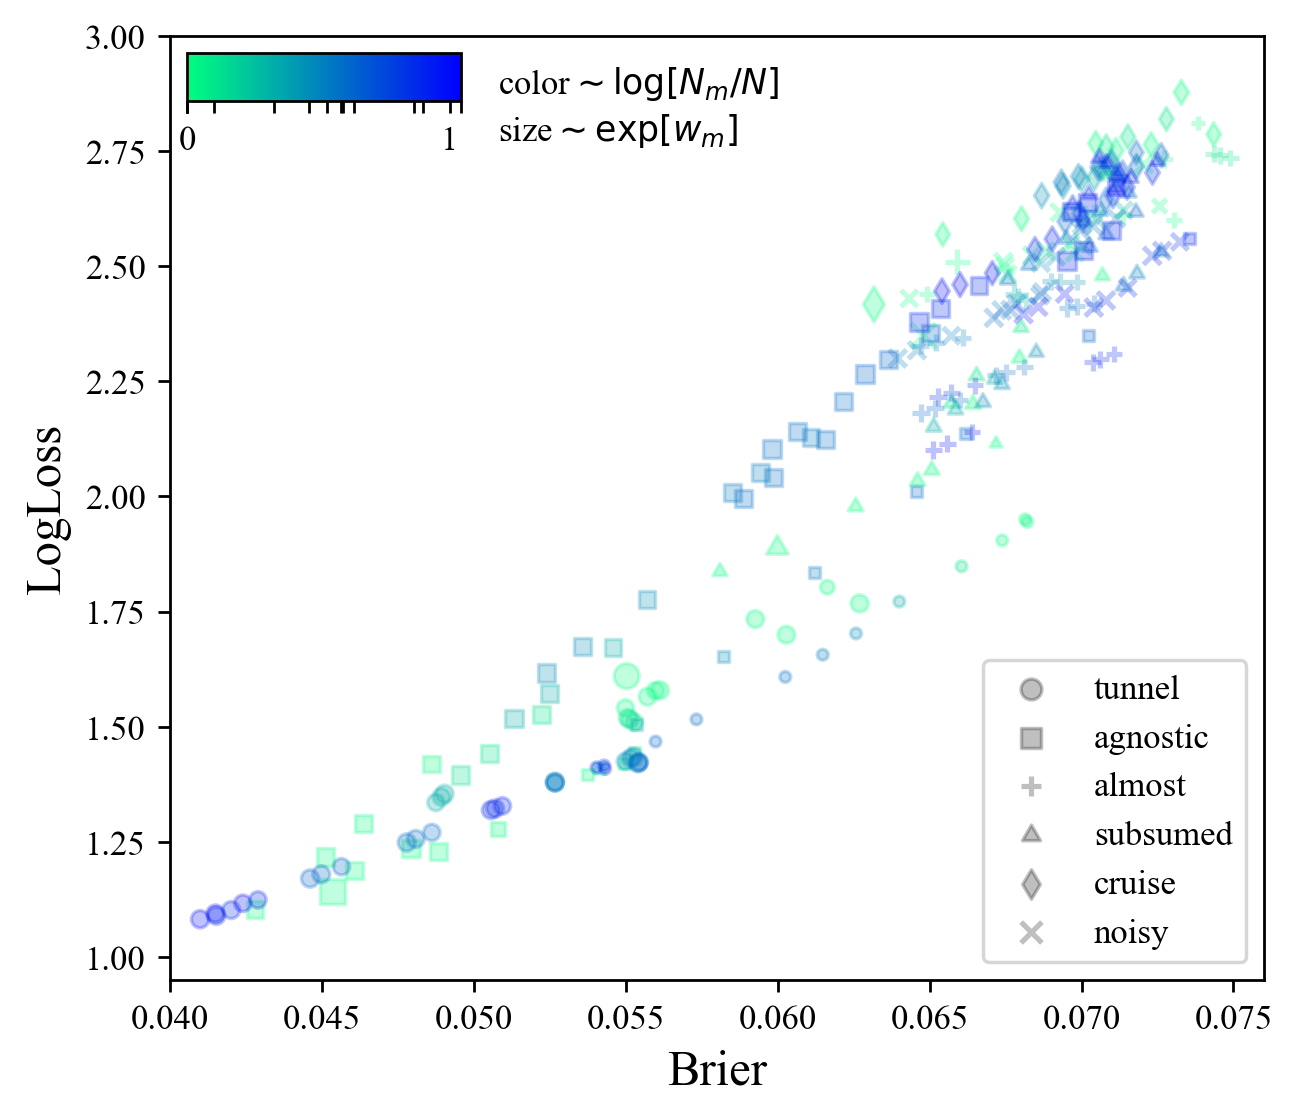
\includegraphics[width=0.5\textwidth]{./fig/all_effects_isolated.png}
% 		\caption{Population-weighted log-loss and Brier scores for classifiers with one class affected by a systematic, as a function of the population of the affected class.
% 		Each point corresponds to an almost perfect classifier that with one class instead affected by a systematic (shape), with log-loss on the $y$ axis and Brier score on the $x$ axis.
% 		The metrics are calculated with a weighting (color and size) proportional to the log of its weight in a weighted average following Equation~\ref{eq:weightavg}.
% 		}
% 	\end{center}
% 	\label{fig:popweight}
% \end{figure}

% The tunnel vision classifier has a consistently low value under the Brier score and log-loss metric (bottom left corner of the plot), only increasing its Brier score once the weighting drops (less blue).
% In this view, the Brier score appears to be more susceptible to tunnel vision than the log-loss, demonstrating a more significant decrease as the size of the affected class increases, but both metrics have concerning behavior in this regard.
% This finding suggests that weighting alone may not be sufficient to counter the influence of this effect, and indicates a need for another balancing mechanism, such as requiring a threshold metric value on all classes.
% When considering a method of converting from one of these metrics to a finall `winner' of the classification challenge, care must be taken to ensure that all approaches do reasonably well at classifying more than one object.
% This thresholding procedure is discussed in the text

% \textbf{Ashish to reaplce/add more here?}
%\aim{Preliminary results indicate weighting will be very important for preventing the tunnel vision classifier from winning. It may be necessary to a priori anticipate which classes will have to be most strongly protected from this systematic via upweighting them.}

%\begin{figure}
%	\begin{center}
%		% 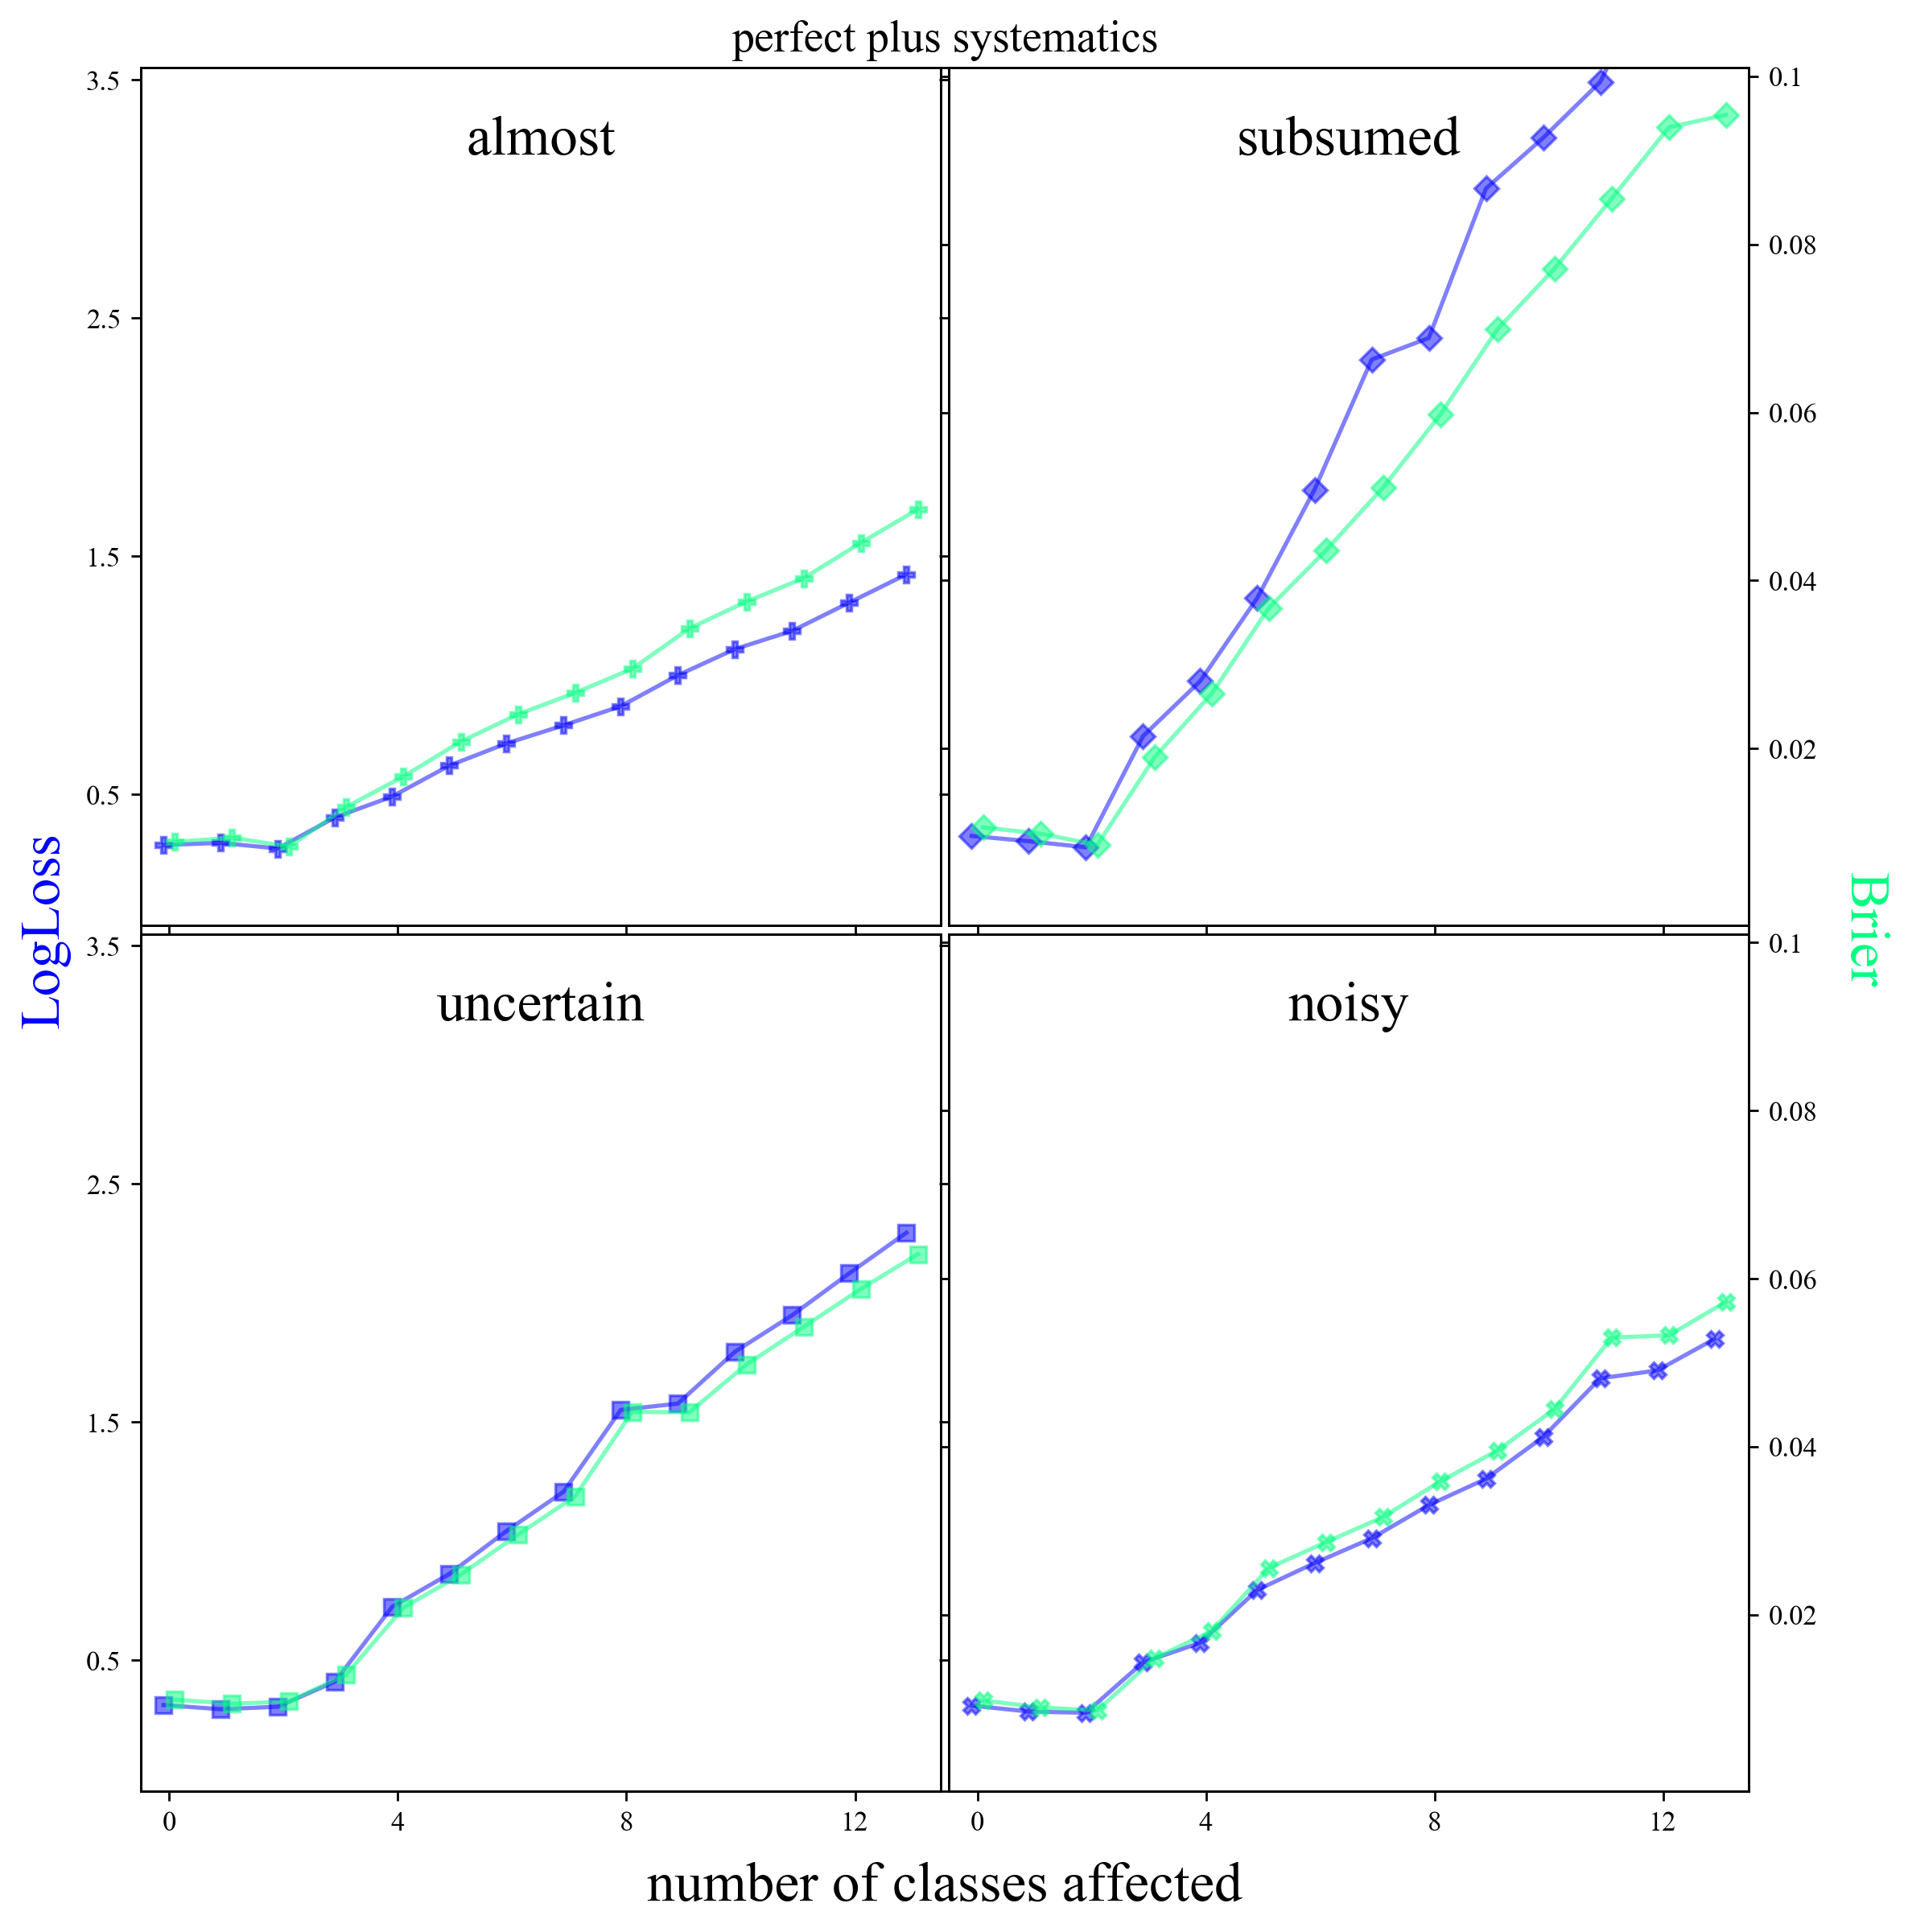
\includegraphics[width=0.5\textwidth]{./fig/systematics_onlyperfect.png}
%		\caption{\aim{After much iteration on how best to present these tests, a figure similar to Figure~\ref{fig:cruise} but for the tunnel vision classifier (heading) on different baseline classifications (panels) as a function of weight on the affected class (rather than number of classes) is under construction.}}
%		\label{fig:tunnel}
%	\end{center}
%\end{figure}

\subsection{Representative classifications}
\label{sec:realresults}

We apply the log-loss and Brier metrics to the classification output from \snmachine. While the classification methods described in \citet{lochner_photometric_2016} refer to the idealized subset of the \snphotcc\ data, these approaches are the state-of-the-art in classification of extragalactic transients.
We present in \sout{Table~\ref{fig:snmachineresults}}\changes{Figure~\ref{fig:snmachineresults} the rankings under the} log-loss and Brier score metrics assuming an equal weight per object.
%, for classification probabilities derived from running the algorithms of \citet{lochner_photometric_2016} on the \snphotcc\ data of Section~\ref{sec:realdata}.
\sout{Table~\ref{fig:snmachineresults} also contains the ranking of classifier performance under each metric.}

% \sout{\begin{table*}[]
% 	\begin{centering}
% \begin{tabular}{lllllll}%ll}
% Rank $R$ & $R_\mathrm{FoM}$ & FoM & %$R_\mathrm{AUC}$ & AUC &
% $R_\mathrm{LogLoss}$ & Log-loss & $R_\mathrm{Brier}$ & Brier \\
% \hline
% 1  & TBDT & 0.635  %& TBDT & 0.982
% & TBDT & 0.0907 & TBDT & 0.0486 \\
% 2  & WBDT & 0.591  %& WBDT & 0.978
% & TSVM & 0.113  & TSVM & 0.0583 \\
% 3  & TSVM & 0.514  %& TSVM & 0.969
% & TNN  & 0.125  & TNN  & 0.0650 \\
% 4  & WSVM & 0.499  %& WSVM & 0.968
% & WSVM & 0.1316 & WBDT & 0.0689 \\
% 5  & TNN  & 0.496  %& TNN  & 0.954
% & WBDT & 0.1321 & WSVM & 0.0730 \\
% 6  & WNN  & 0.480  %& WNN  & 0.946
% & TKNN & 0.146  & WNN  & 0.0750 \\
% 7  & TKNN & 0.384  %& TKNN & 0.942
% & WNN  & 0.152  & TKNN & 0.0787 \\
% 8  & TNB  & 0.340  %& WKNN & 0.894
% & WKNN & 0.228  & TNB  & 0.105  \\
% 9  & WKNN & 0.114  %& TNB  & 0.879
% & TNB  & 0.251  & WKNN & 0.132  \\
% 10 & WNB  & 0.0365 %& WNB  & 0.850
% & WNB  & 0.443  & WNB  & 0.178  \\
% \end{tabular}
% 	\caption{
% 	The values of three metrics for each of ten \snmachine\ classifiers with equal weight per object.
% 	The metrics broadly agree on the ranking of the classifiers, confirming consistency between a conventional metric of classification performance and the metrics of probabilistic classifications presented here.
% 	However, there are some differences with pairwise swapping between the log-loss and Brier rankings and some significant reordering of ranks 2 through 5 with the FoM metric relative to the probabilistic metrics.
% 	}
% 	\label{tab:snmachineresults}
% 	\end{centering}
% \end{table*}}

\begin{figure}
	\begin{center}
		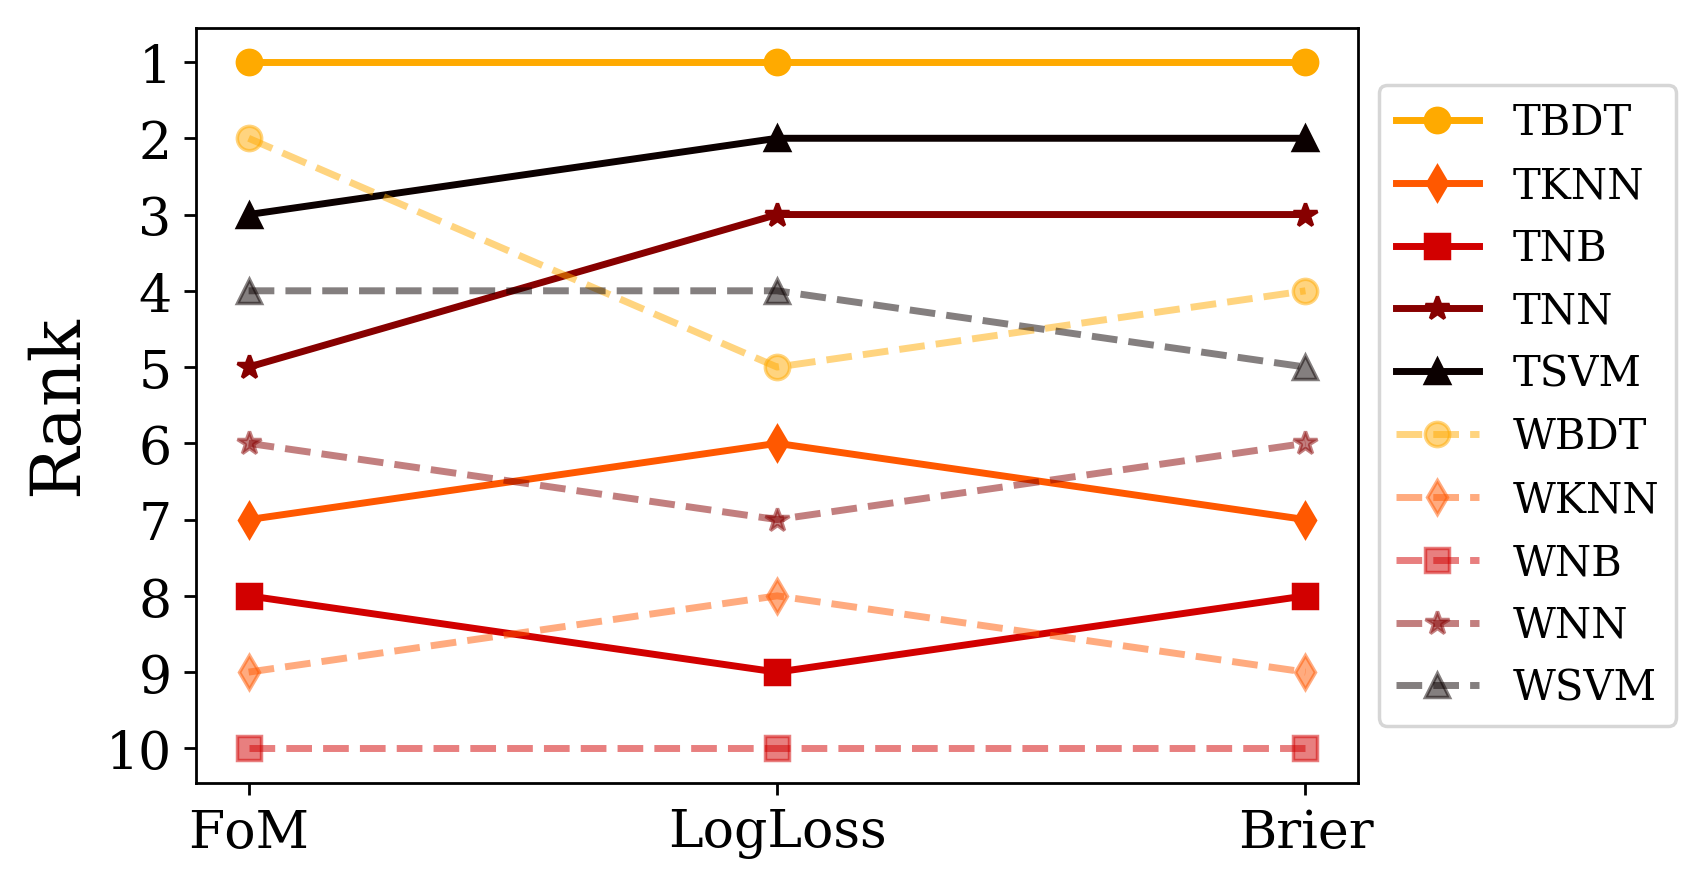
\includegraphics[width=0.49\textwidth]{./fig/Tables3_option4.png}
		\caption{
		\changes{The rankings of each of the five \snmachine\ classification algorithms (Boosted Decision Tree (BDT), K-Nearest Neighbors (KNN), Naive Bayes (NB), Neural Network (NN), and Support Vector Machine (SVM)) on template (T*) and wavelet (W*) features with equal weight per object under the three metrics.
		The metrics broadly agree on the ranking of the classifiers, confirming consistency between a conventional metric of classification performance and the metrics of probabilistic classifications presented here.
		However, there are some differences with pairwise swapping between the log-loss and Brier rankings and some significant reordering of ranks 2 through 5 with the FoM metric relative to the probabilistic metrics.}
		}
	\end{center}
	\label{fig:snmachineresults}
\end{figure}

We apply our metrics to the classification output from \snmachine\ applied to the \snphotcc\ dataset as an example of representative light curves and representative classifiers used in extragalactic astronomy.
We present in \sout{Table~\ref{fig:snmachineresults}}\changes{Figure~\ref{fig:snmachineresults}} the rankings of each classifier under the log-loss and Brier scores assuming an equal weight per object, as well as the original \snphotcc\ metric described in Section~\ref{sec:deterministic}.
\sout{Table~\ref{fig:snmachineresults} also contains the ranking of classifier performance under each metric.}

The Brier score, log-loss, and \snphotcc\ FoM are in agreement as to the first- and last-ranked classifiers.
This consensus indicates that both of the potential \plasticc\ metrics are roughly consistent with our intuition about what makes a good classifier, providing an anchor between accepted notions of an appropriate metric and the metrics of probabilistic classifications under consideration here.
One should be careful not to generalize, however, as the rankings under the three metrics are not identical.

We note that the FoM differs more from the Brier score and log-loss metrics than they do from one another.
This is perhaps unsurprising, given that the \snphotcc\ was specifically looking to value classification algorithms that were pure (that yielded a large number of SNIa classifications and few interlopers from the other classes), as opposed to metric that rewards good performance across classes.
